\chapter{\uppercase{Implementation}}

\section{\uppercase{Overview}}

Phase 1 implements a practical, production-minded prototype of the Multi-Stage Code Security Framework. The implementation combines a fast Tree-sitter based syntactic engine for rapid filtering with a CodeQL-backed semantic pipeline that produces Code Property Graphs (CPGs) suitable for future graph-learning work. The pipeline is designed to be incremental, observable, and modular: each stage emits normalized artifacts that downstream stages consume.

Figure~\ref{fig:pipeline} shows the Phase-1 pipeline architecture.

\begin{figure}[H]
\centering
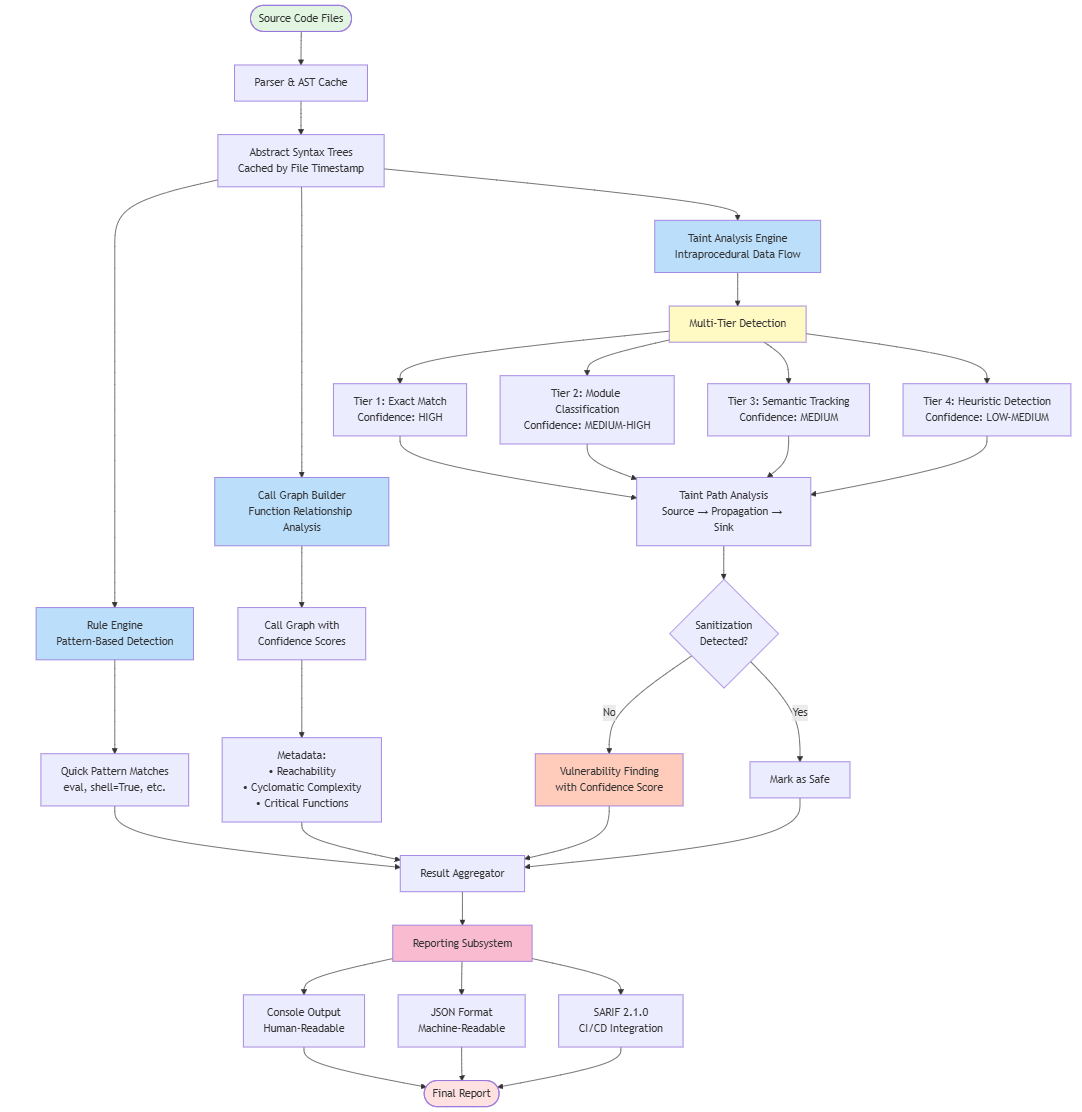
\includegraphics[width=0.75\textwidth]{Figures/implementation.png}
\caption{High-level Pipeline}
\label{fig:pipeline}
\end{figure}

\section{\uppercase{Engineering Goals and Constraints}}

Implementation decisions prioritized:

\begin{itemize}
    \item \textbf{Determinism \& reproducibility} : analyses must produce repeatable findings given the same inputs and environment.
    \item \textbf{Incrementality} : re-parse only changed files; reuse cached ASTs/graphs where possible.
    \item \textbf{Performance} : sublinear end-to-end wall time for typical scans via parallelism and cache layers.
    \item \textbf{Transparency} : output traceable taint paths and the CPG fragments referred to by each finding.
    \item \textbf{Extensibility} : intermediate artifacts serialized in neutral formats to enable GNN and LLM components later.
\end{itemize}

Constraints included limited engineering time, reliance on third-party extractors for deep semantic analysis (CodeQL), and an explicit Phase-1 scope that avoided full interprocedural taint summarization.

\section{\uppercase{Input Processing and AST Caching}}

\subsubsection{Parsing Pipeline}

Input discovery walks the repository root and applies a configurable inclusion/exclusion pattern (glob-based). Language detection is performed per-file.

Each source file is parsed into a concrete AST using an incremental parser. Parsers are deterministic and stable with respect to whitespace and comments to enable exact location mappings.

\subsubsection{AST Cache Design}

\begin{itemize}
    \item \textbf{Cache key:} \texttt{\{file-path\}:\{file-size\}:\{mtime-iso\}:\{parser-version-hash\}}
    \item \textbf{Cached value:} serialized AST + lightweight symbol summary (imports, top-level defs, exported names)
    \item \textbf{Cache storage:} per-project directory cache (on-disk) with an in-memory LRU for the current run
    \item \textbf{Cache invalidation:} TTL policy + explicit invalidation when parse errors or configuration changes occur
\end{itemize}

\subsubsection{Complexity \& Performance}

Parsing cost is roughly linear in source length:
\begin{equation}
T_{\text{full parse}} = O(|S|)
\label{eq:full_parse}
\end{equation}

With caching, only changed files re-parse. For incremental edits, the cost becomes:
\begin{equation}
T_{\text{incremental}} = O(|\text{changed\_region}| + \text{overhead})
\label{eq:incremental_parse}
\end{equation}

where $|\text{changed\_region}| \ll |S|$, and average-case work is $O(k + m)$ with $k$ nodes re-used and $m$ the size of the re-parsed fragment. This results in amortized near-constant time per incremental change for large repos.

\section{\uppercase{Declarative Rule Engine (Tree-sitter SAST)}}

\subsubsection{Rule Format and Compilation}

Rules expressed in declarative YAML with the following fields:
\texttt{id}, \texttt{title}, \texttt{severity}, \texttt{patterns} (AST shape), \texttt{confidence\_hint}, \texttt{examples}, \texttt{remediation}.

Before execution, rules are validated and compiled into optimized AST matcher objects that use selector paths rather than naive tree traversal to reduce matching cost.

\subsubsection{Matcher Capabilities \& Engine Flow}

\textbf{Predicate categories:} syntactic node shape, import/module context, identifier resolution, literal regex, and simple local dataflow predicates (e.g., arg index tainted).

\textbf{Execution:} depth-first matching with short-circuiting; rule hits produce \texttt{Finding} objects immediately for subsequent aggregation.

\subsubsection{Finding Object Model}

Canonical fields emitted by SAST stage:

\begin{itemize}
    \item \texttt{finding\_id} --- unique id
    \item \texttt{rule\_id}, \texttt{title}, \texttt{severity}
    \item \texttt{location} --- file, line range, column range, snippet hash
    \item \texttt{confidence} --- numeric (0.0--1.0)
    \item \texttt{trace} --- optional node IDs pointing into the CPG fragment
    \item \texttt{remediation\_text}, \texttt{refs} --- links to OWASP/CWE or docs
\end{itemize}

\subsubsection{Performance}

Typical pass runs in:
\begin{equation}
T_{\text{rules}} = O(N_{\text{rules}} \times C_{\text{match}})
\label{eq:rule_complexity}
\end{equation}

where $C_{\text{match}}$ is the cost of matching per rule. With pruning and compiled matchers keeping wall time low, empirically the SAST pass provided sub-second feedback for single-file scans and an order-of-magnitude speed improvement over unoptimized pattern checks.

\section{\uppercase{Structural Analysis and Call Graph}}

\subsubsection{Symbol Extraction}

After parsing, the pipeline builds a project-wide symbol index that maps identifiers to fully qualified definitions with scope metadata (module, class, function). The index supports incremental updates.

\subsubsection{Call Graph Construction}

\textbf{Algorithm:}

\begin{enumerate}
    \item For each function body, enumerate call expression nodes.
    \item Resolve callee using symbol index + import alias map; when resolution fails, record a dynamic call placeholder.
    \item Create directed edge \texttt{caller → callee} annotated with location, \texttt{call\_syntax}, and \texttt{resolution\_confidence}.
\end{enumerate}

\textbf{Edge confidence heuristic:}

\begin{equation}
C_{\text{edge}} = \begin{cases}
1.0 & \text{direct definition in same module} \\
0.9 & \text{imported from project module} \\
0.7 & \text{third-party library} \\
0.5 & \text{dynamic/unresolved (getattr/higher-order)}
\end{cases}
\label{eq:edge_confidence}
\end{equation}

\subsubsection{Queries Supported}

\begin{itemize}
    \item \textbf{Reachability from entry points:} BFS with early stopping on visited nodes
    \item \textbf{Critical path computation:} shortest/most central paths from entry points to sink nodes
    \item \textbf{Cycle detection:} Tarjan's algorithm for strongly connected components (SCCs)
\end{itemize}

\subsubsection{Data Export}

Call graph is stored as a compact adjacency list with metadata and optionally exported as GraphML or DOT for visualization and as DGL node/edge tables when generating CPGs.

\section{\uppercase{Intraprocedural Taint Engine --- Algorithm and Pseudocode}}

Phase 1's taint engine performs flow-sensitive, path-insensitive intraprocedural analysis. The following is an abstract outline and key design choices.

\subsubsection{Data Structures}

\begin{itemize}
    \item \texttt{TaintState}: mapping \texttt{identifier → TaintLabel}
    \item \texttt{TaintLabel} = $\{\text{tainted\_sources}: \mathcal{P}(\text{source\_ids}), \text{confidence}: [0,1], \text{sanitizers}: \mathcal{P}(\text{sanitizer\_ids})\}$
    \item \texttt{TaintPath}: list of $(\text{node\_id}, \text{operation}, \text{label})$ describing propagation from source→sink
    \item \textbf{Source/Sink/Sanitizer catalog:} declarative registry with tiers and confidence hints
\end{itemize}

\subsubsection{Propagation Rules (Forward Single-Pass)}

\begin{enumerate}
    \item \textbf{Initialization:} Mark parameters and immediate expressions from recognized source sites as tainted.

    \item \textbf{Assignment:} \texttt{x = expr} → \texttt{TaintState[x] = combine\_taint(expr)}

    The taint combination function unions taint sets:
    \begin{equation}
    \text{combine\_taint}(\text{expr}) = \bigcup_{v \in \text{vars}(\text{expr})} \text{TaintState}[v]
    \label{eq:taint_combine}
    \end{equation}

    Confidence computation uses maximum:
    \begin{equation}
    C_{\text{taint}}(x) = \max_{v \in \text{vars}(\text{expr})} C_{\text{taint}}(v)
    \label{eq:taint_confidence}
    \end{equation}

    \item \textbf{Operation propagation:} for \texttt{x = y + z} or \texttt{x = f(y)}: propagate taint from operands/args to \texttt{x}. For known library functions, apply function-specific transfer rules.

    \item \textbf{Call handling:}
    \begin{itemize}
        \item If callee is in known sanitizer list → attempt to clear taint on returned value (reduce confidence)
        \item If callee is unknown → assume taint preserved for arguments that are passed to sinks; conservatively assume return may be tainted
    \end{itemize}

    \item \textbf{Branch merging:} when control-flow joins, merge TaintStates using union semantics:
    \begin{equation}
    \text{TaintState}_{\text{merge}} = \text{TaintState}_{\text{if}} \cup \text{TaintState}_{\text{else}}
    \label{eq:state_merge}
    \end{equation}

    Label confidence becomes maximum or a defined fusion function.

    \item \textbf{Sink detection:} when a sink is invoked and an argument is tainted, create \texttt{TaintPath} and a \texttt{Finding} with confidence derived from:
    \begin{itemize}
        \item detection tier (exact/module/semantic/heuristic)
        \item taint propagation confidence along path
        \item call graph reachability (distance weighting)
        \item analyzer agreement (if rule engine also flagged)
    \end{itemize}
\end{enumerate}

\subsubsection{Pseudocode (Simplified)}

\begin{algorithm}[H]
\caption{Intraprocedural Taint Analysis Algorithm}
\label{alg:taint_algo}
\begin{algorithmic}[1]
\Function{AnalyzeFunction}{func\_ast}
    \State $state \gets \text{TaintState()}$
    \ForAll{$stmt \in func\_ast.statements$}
        \If{$is\_assignment(stmt)$}
            \State $rhs\_label \gets eval\_expr\_taint(stmt.rhs, state)$
            \State $state[stmt.lhs] \gets merge\_labels(state.get(stmt.lhs), rhs\_label)$
        \ElsIf{$is\_call(stmt)$}
            \State $callee \gets resolve\_callee(stmt)$
            \State $arg\_labels \gets [eval\_expr\_taint(a, state) \text{ for } a \in stmt.args]$
            \If{$is\_sink(callee)$ \textbf{ and } any($l.is\_tainted()$ \textbf{ for } $l \in arg\_labels$)}
                \State $record\_finding(build\_taint\_path(arg\_labels, stmt), compute\_confidence(\dots))$
            \EndIf
            \If{$is\_sanitizer(callee)$}
                \State $apply\_sanitizer\_effects(state, stmt)$
            \EndIf
        \ElsIf{$is\_control\_flow(stmt)$}
            \State $saved\_state \gets state.copy()$
            \State $state\_if \gets analyze\_block(stmt.if\_block, state.copy())$
            \State $state\_else \gets analyze\_block(stmt.else\_block, state.copy())$
            \State $state \gets merge\_states(state\_if, state\_else)$
        \EndIf
    \EndFor
    \State \Return $collected\_findings$
\EndFunction
\end{algorithmic}
\end{algorithm}

\subsubsection{Detection Tiers \& Confidence Composition}

Confidence computation is multiplicative/weighted. Let:

\begin{itemize}
    \item $T$ be tier confidence $\in (0,1]$ depending on detection tier:
    \begin{equation}
    T = \begin{cases}
    T_e = 0.95 & \text{exact match} \\
    T_m = 0.85 & \text{module classification} \\
    T_s = 0.80 & \text{semantic tracking} \\
    T_h = 0.60 & \text{heuristic detection}
    \end{cases}
    \label{eq:tier_confidence}
    \end{equation}

    \item $P$ be path confidence $\in (0,1]$ derived from taint propagation. For a taint path with $n$ edges having per-edge confidences $e_i \in (0,1]$:

    \textbf{Option A (multiplicative):}
    \begin{equation}
    P = \prod_{i=1}^{n} e_i
    \label{eq:path_mult}
    \end{equation}

    \textbf{Option B (weighted geometric mean):}
    \begin{equation}
    P = \exp\left(\frac{1}{n} \sum_{i=1}^{n} \ln e_i\right)
    \label{eq:path_geom}
    \end{equation}

    Phase 1 used Option B to avoid exponential decay on longer but still reliable paths.

    \item $R$ be reachability factor $\in (0,1]$, based on call-graph distance from entry point:
    \begin{equation}
    R = \begin{cases}
    1.0 & \text{directly reachable from entry} \\
    \alpha^k & \text{reachable through } k \text{ calls, } \alpha = 0.9 \\
    0.5 & \text{unreachable (deprioritization)}
    \end{cases}
    \label{eq:reachability}
    \end{equation}

    \item $A$ be analyzer agreement bonus $\in [1.0, 1.2]$, multiplicative factor if multiple analyzers independently detect same issue.
\end{itemize}

Final fused confidence:
\begin{equation}
C = \min\left(1.0, T \cdot P^\beta \cdot R^\gamma \cdot A\right)
\label{eq:confidence_final}
\end{equation}

where $\beta$ and $\gamma$ are tuning exponents (Phase 1 used $\beta = 0.75$, $\gamma = 0.5$). These are tunable via configuration.

\section{\uppercase{CodeQL Integration and CPG Construction}}

\subsubsection{Why CodeQL}

CodeQL provides a mature interprocedural extractor and a queryable relational database of program facts, accelerating the production of semantically rich artifacts. It was used to generate a canonical database that was then converted to a CPG suitable for downstream GNN processing.

\subsubsection{Conversion Pipeline (Detailed Steps)}

\begin{enumerate}
    \item \textbf{Extraction:} run the CodeQL extractor to produce a code database containing AST, call relationships, dataflow facts, and queryable entities.

    \item \textbf{Relational queries:} execute a set of CodeQL queries to export nodes (functions, variables, calls) and edges (AST\_CHILDS, CFG\_NEXT, DFG edges, CALL).

    \item \textbf{Normalization:} map CodeQL entities into a uniform CPG schema of typed nodes and edges, preserving location metadata and source hashes.

    \item \textbf{Feature augmentation:} attach per-node features such as tokenized code snippets, normalized identifiers, cyclomatic complexity, centrality metrics, and tier hints (e.g., node likely to be source/sink).

    \item \textbf{Hetero-graph assembly:} build a DGL-compatible heterogeneous graph with node/edge types matching the CPG schema.

    \item \textbf{Serialization:} store CPG fragments per-file in compressed format for later batch training or inference.
\end{enumerate}

\subsubsection{Statistics \& Sizing}

Typical function-level CPGs in Phase 1 contained 10--50 nodes and 30--200 edges. A medium module produced 1k--10k nodes depending on code density and third-party integrations.

\section{\uppercase{Reporting, Standard Formats, and CI Integration}}

\subsubsection{Normalizing Findings}

All findings (SAST / Taint / CodeQL) are normalized into the canonical \texttt{Finding} model described earlier. This enables consistent downstream filtering and sorting.

\subsubsection{SARIF Mapping}

Findings are exported as SARIF 2.1.0 with:
\texttt{ruleId}, \texttt{level} (error/warning/note), \texttt{locations} (region), \texttt{message.text}, \texttt{properties} (confidence, tiers, taint-path as JSON).

CI integration uses exit codes:

\begin{equation}
\text{exit\_code} = \begin{cases}
0 & \text{no findings above configured severity} \\
1 & \text{critical/high findings detected} \\
2 & \text{medium/low findings detected}
\end{cases}
\label{eq:exit_codes}
\end{equation}

The SARIF output enables native integration with code scanning dashboards (e.g., GitHub).

\subsubsection{Result Aggregation and De-duplication}

Aggregator merges overlapping findings using a canonicalization key:
\begin{equation}
K_{\text{canon}} = \text{hash}(\text{file}, \text{start\_line}, \text{end\_line}, \text{rule\_signature})
\label{eq:dedup_key}
\end{equation}

Duplicate findings from multiple analyzers are fused; evidence sources are combined into a single finding with a computed aggregated confidence.
